\documentclass{article}
\usepackage{graphicx}
\usepackage{subfig}
\usepackage{amsmath}
\begin{document}
\section{Introduction}
\subsection{Motivation: CETD use new designed component, the formal security is not provided with the design}
Message authentication code(MAC) is a cryptographic primitive to protect the integrity of message transmitted between sender and receiver. Message blocks are adopted to a MAC scheme as input and a short message block, called tag in majority of research works, is generated as output. The tag is concatenated to the input message blocks and this data-tag pair is used as unit in transmission. Early MAC schemes are symmetric-keyed, stateless(secrete key is the only resource of randomness in tag generation) and constructed with block cipher. As stateless MAC schemes suffer from replay attacks, MAC schemes using state information of message blocks protected as additional information in tag generation have been designed.

Hong, Guo and Hu \cite{keylist}introduced a cost-effective tag design for integrity protection, specially for embedded systems. The MAC scheme adopted is an original design with state constructed with two components: bit segments swap and block-level rotate shift. When generating a tag, a nonce generated by encrypting a tuple(message address, counter, random number) is used as additional input in processing the input data for swap and shift components. 

In \cite{keylist}, a security analysis of the MAC scheme adopted in cost-effective tag design is provided by indicating that tag generated is random under brute-force attack. This evaluation procedure contains the following weakness:
\begin{itemize}
	\item The capability of the adversary is not depicited clearly
	\item The security result under each type of attack in the threat model is not provided
	\item The data processing components used in constructing the MAC scheme in cost-effective tag design are not cryptographic primitives, the security assumption of these components are unclear.
	\item The evaluation procedure does not belong to any common formal evaluation framework. The security result provided can not be used in comparison with the formal results from evaluation of other MAC schemes
\end{itemize}
The tag design from Hong et al. showed reduction of on-chip, performance and memory overhead. This cost advantage attracted us to research its security with a formal approach.
\subsection{Approach: Analysis the security of CETD with computational model}
In this article, we will show that from the viewpoint of computational model based security analysis, the secure block cipher used in generating nonce can not ensure the security of Cost-Effective Tag Design as a message authentication system under several attacks. To make this statement meaningful, we follow the well recognized security notions of message authentication system in computational model.
\subsection{Results: found security weakness, security optimization and results for optimized design }
\subsection{Approach: Security Analysis based on Computational Model}


\section{Preliminary}
\subsection{Security of Message Authentication Systems}
\paragraph{Message Authentication System}
In the scenario of processor-memory architecture, data integrity refers to maintaining the data on the transmission outside the chip and stored on off-chip memory untampered. If the data stored on off-chip memory is modified, or some external data is  injected to the system S, we can say that the data integrity of S is attacked. If the system S can not examine the tampered data or injected data, the attack is assumed to be successful. According to our knowledge, there are two aspects of attacks on data integrity:
\begin{enumerate}
	\item Introducing new content: The content of data in the system is modified, or data construct by the attacker is inserted to the system.
	\item Replacing data with valid copy: The data D in transmission or on the memory is replace with the following two types of copy: A copy of D at an old time point or a copy of other data from different memory address.
\end{enumerate}

The goal of integrity protection can be defined as the capability to examine whether the data to read by processor has been tampered. Cryptographic hash function and Message Authentication Code(MAC) scheme are common cryptographic primitives aiming to protect the data integrity of a system. These theoretical models for integrity protection are called Authentication Primitives(AP) in some research works.

Hash is a short message block computed by hash function with data block D as input.
When processor writes a data block to a memory address, the data block D is sent to Hash function and a Hash value H1 is computed and stored on the chip. The hash value H is stored on chip following the order of data block on the memory. The message stored on the memory from chip is data block D alone.
When the processor wants to read a data block D from memory, D is sent to hash function and an hash value H2 is computed. If H1 is identical to H2, then the data block D is assumed to be untampered and read by processor.
Figure 3-a expresses functionality of hash function in integrity protection.
If the integrity of a processor-memory system is protected by hash function, the possible attacks are:
\begin{enumerate}
	\item Modify the content of a data block
	\item Insert new data
	\item Replace the content of a data block with a copy of data from other address
\end{enumerate}
If using hash function to protect integrity, the three attacks in the above list can be defended if the hash function behave like an theoretical random function, which means for any input data block D, its hash value H is randomly assigned.

\begin{figure}[htbp]
\centering
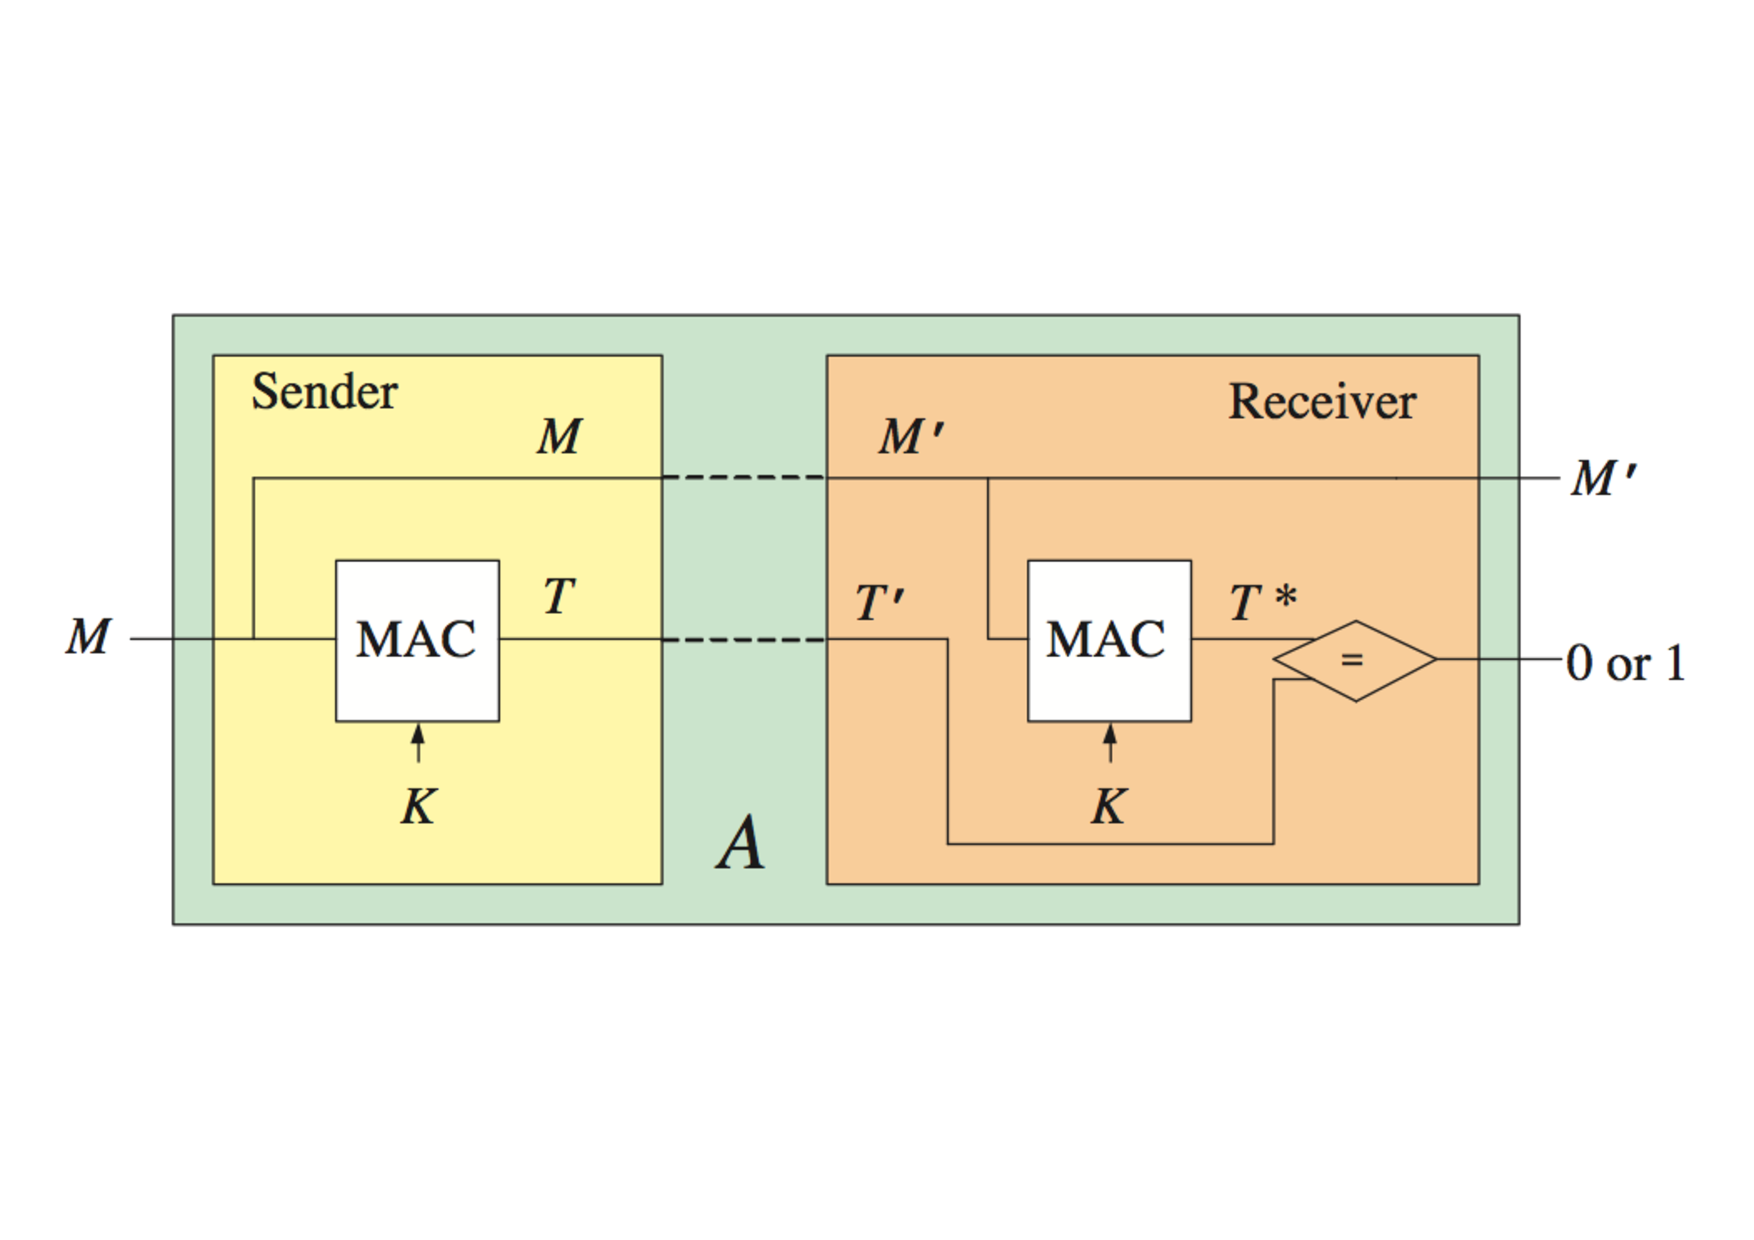
\includegraphics[scale=0.4]{./diagrams/MAC.pdf}
\caption{The Concept of Deterministic MAC Scheme}
\label{deterministic_mac }
\end{figure}
Message Authentication Code(MAC), called tag in some research works, is a short message block. A tag is generated by a MAC scheme by accepting a data block D as input and process D with a secret key K inside the scheme. The MAC schemes require only secrete key to process inputs are denoted as deterministic MAC schemes in some research works.
Some MAC schemes require an additional input block, named nonce, in the generation of tag. Nonce is used to provide uniqueness for each input invoking the MAC scheme. MAC schemes with nonce as additional input are called state MAC schemes in some research works.
When the processor writes a data block D to the memory, MAC scheme computes a tag  and concatenate the tag withe data forming a data-tag pair. The data-tag pair is sent to off-chip memory for storage.
When the processor reads a data from memory, the data-pair is sent to the chip and to MAC scheme. Assume the data part is D and tag part is T1. MAC scheme compute a tag T2 using D T2 is compared with T1. If T1 is identical to T2, D is assumed to be untampered.
 Figure 3-b expresses the functionality of MAC scheme in integrity protection.
If the integrity of a processor-memory system is protected by MAC scheme, the possible attacks are:
\begin{enumerate}
	\item Modify the content of a data-tag pair
	\item Insert new data-tag pair
	\item Replace the content of a data-tag pair with a copy of data-tag pair from other address
	\item Replace the content of a data-tag pair with a copy of this pair in an old time point
\end{enumerate}
If a MAC scheme is capable to defend the 1st and 2nd attacks in the list, it should ensure that for any data block D, the tag is randomly assigned. If this scheme is capable to defend the 3rd and 4th attacks too, it should ensure for any two identical data blocks D1 and D2 that are written to memory on different time or to different addresses, their tags T1 and T2 should be randomly generated.

\subsection{Security Analysis on Message Authentication Systems}
\paragraph{Security Notion of Message Authentication Systems}
 According to our knowledge, there have been three categories of security evaluation mechanisms designed, namely computational model based on provable security theory, dolev-yao model based on formal methods theory and automatic security analysis framework combining the advantages from previous two models.
\paragraph{Symbolic Model based Security Analysis}

\paragraph{Computational Sound Security Analysis based on Symbolic Model}
\paragraph{Computational Model based Security Analysis}

\paragraph{Security Notion of Message Authentication Systems in Computational Model}
From the viewpoint of computational model, the security of a message authentication system can be broken If the resources, such as computation time, is unlimited for the attacker, and AP system can always be broken at some time. Research works on security analysis on AP system try quantify the evaluation result under the assumption that the attack has limitation on computation resources.
\paragraph{Code-based Game-Playing Techniques}
In cryptography, a viewpoint of game-playing proofs represents the technique that abstracts the interaction between the adversary and environment to a program named game. Computing the probability of adversary becomes the stepwise refinement of a sequences of games. 
The application of this viewpoint of game-playing proofs in security analysis began with the article "Probabilistic encryption" from Goldwasser and Micali\cite{keylist}, and "Theory and applications of trapdoor functions" from Yao \cite{keylist}and then adopted in the security analysis of various encryption systems\cite{keylist}.  

In "How to protect DES against exhaustive key search", Kilian and Rogaway modeled a game with diciplines to a piece of code and introduced the idea of code-base game-playing proofs, which has been applied in encryption and authentication systems analysis. 
\begin{itemize}
	\item The benifits of modeling a game to code is xxxxxxxx.
	\item The procedure of applying code-based game-play in analyzing security of message authentication system
	\item 
\end{itemize}

  

\paragraph{Cost-Effective Tag Design}

\end{document}